\documentclass[10pt,twocolumn,letterpaper]{article}

%%%%%%%%% PAPER TYPE  - PLEASE UPDATE FOR FINAL VERSION
\usepackage[review]{cvpr}      % to produce the REVIEW version
%\usepackage{cvpr}             % to produce the CAMERA-READY version
%\usepackage[pagenumbers]{cvpr} % to force page numbers, e.g. for an arXiv version

\usepackage{graphicx}
\usepackage{amsmath}
\usepackage{amssymb}
\usepackage{booktabs}
\usepackage{enumitem}
\usepackage{xcolor}

\definecolor{cvprblue}{rgb}{0.21,0.49,0.74}
\usepackage[pagebackref,breaklinks,colorlinks,allcolors=cvprblue]{hyperref}

\def\paperID{*****}
\def\confName{CVPR}
\def\confYear{2027}

\begin{document}

\title{Pixel Art Is a Palette, Not a Downscale:\\Rebuilding Targets and Decoding for Tiny Sprite Generation}

\author{Anonymous CVPR submission\\
Paper ID \paperID}

\maketitle

\begin{abstract}
Text-to-image models fail at the smallest images people draw on purpose: 12--24\,px RGBA game sprites, where a handful
of colours and hard alpha edges are the medium. We show that the usual failure is not a modelling failure but a target
failure. In the sprite corpus this area trains on, only 7.1\% of the images are natively 16\,px or smaller; the rest is
25--64\,px artwork box-downscaled into the low-resolution buckets, and 4{,}888 pixel-identical duplicates leave a twin
in training for 16.2\% of the held-out set. A model fitted to those targets learns soft, fifty-colour blobs, and the
evaluation reference, drawn from the same pool, rewards exactly that. We rebuild the targets and evaluate against
references that contain only real low-resolution pixel art. Under this protocol the data work alone takes FD-DINOv2
from 167.2 to 117.9 at 16\,px. We then close the remaining gap where it actually lies: real sprites use a median of six
opaque colours while every sampling rule we tested emits more than fifty. Projecting the predicted $\hat x_0$ onto a
per-sprite $k$-colour palette during the late denoising steps reaches $31.8 \pm 0.5$ --- better than quantising
finished samples (41.6), than one corpus-wide palette (120.1) and than a median filter that removes the same dither
(112.2). The rule is a property of the recipe rather than of the network: a transformer backbone that trails the UNet
by 36.5 FD without it lands within 0.7 with it. Applied to sprites from generators we did not train, it improves native
FD by 36--41\% while preserving 80\% of the silhouette. Against external systems given the same palette post-process we
reach 50.8 versus 134.4 for gpt-image-2 with downscaling.
\end{abstract}

\begin{figure}[t]
\centering
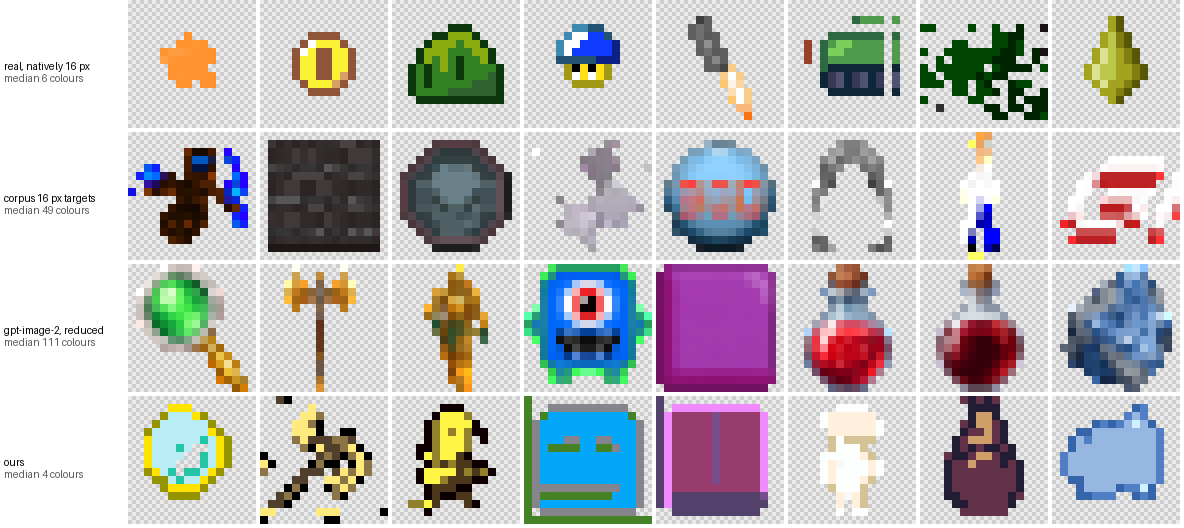
\includegraphics[width=\linewidth]{figures/fig_teaser.png}
\caption{Four rows of 16\,px RGBA sprites, nearest-neighbour magnified, with the median number of opaque colours
per row. Real sprites drawn at this size use six; the corpus's own 16\,px targets, which are 25--64\,px artwork
box-downscaled, use 49; gpt-image-2 rendered large and reduced uses 111; ours uses four. The third row is the
easiest on the eye and the furthest from the medium.}
\label{fig:teaser}
\end{figure}

\section{Introduction}
\label{sec:intro}

Game sprites are among the smallest images anyone draws on purpose: an item or a character on a 12--24\,px RGBA canvas,
built from hard edges, a handful of flat colour regions and a transparent background. At these sizes there is no
texture in which to hide a mistake --- one wrong pixel changes the silhouette, one blended colour reads as blur. The
obvious recipe, prompting a large text-to-image model and shrinking its output, produces something recognisable but not
a sprite: it keeps the soft shading and the hundred-odd colours of an illustration (Figure~\ref{fig:teaser}).

This paper is about a failure one level below the model. We train a dedicated generator for this medium --- a 72.5M
pixel-space diffusion model over RGBA sprites, conditioned on a frozen CLIP text encoder and a resolution-bucket label
--- and find its weaknesses inherited from what it is asked to imitate. In the sprite corpus this area trains on, only
7.1\% of the images are natively 16\,px or smaller; two thirds are 25--64\,px artwork that the pipeline box-downsamples
into the low-resolution buckets, and 4{,}888 pixel-identical duplicates leave a twin in training for 16.2\% of the
held-out set. A model fitted to those targets learns what they are: soft, fifty-colour blobs. Worse, the standard
evaluation reference is drawn from the same pool, so it rewards the blur it caused, and the ranking of methods under it
does not survive contact with real pixel art.

We change both the targets and the yardstick. On the data side we remove the duplicates, forbid feeding a sprite to a
bucket more than $1.5\times$ below its native size, and add 14{,}999 natively small sprites from permissively licensed
collections, captioned with a vision--language model. On the evaluation side we define the \emph{native protocol}:
FD-DINOv2 against real sprites that are natively at most $R$\,px, never downscaled. At 16\,px the data work alone moves
the model from 167.2 to 117.9.

What remains is a property of the medium that continuous diffusion cannot express. Real 16\,px sprites use a median of
six opaque colours and 46\% of their adjacent opaque pixel pairs are exactly equal; every sampling rule we tested emits
more than fifty colours and reaches 8\%, spending the difference on few-level dither inside regions that should be
flat. We close that gap inside the sampler: during the late denoising steps we project the predicted $\hat x_0$ onto a
per-sprite $k$-colour palette (batched $k$-means over the opaque pixels, alpha untouched) and continue, so the
remaining steps repair the seams hard quantisation leaves. At 16\,px this takes FD from 87.1 to $31.8 \pm 0.5$, where
quantising the finished samples reaches only 41.6.

Two results say the rule is not an artefact of our network. Replacing the UNet with a 69.7M transformer, everything
else held fixed, gives a model that trails by 36.5 FD under plain guidance and by 0.7 once the projection is on: the
decoding rule absorbs the difference between the two architectures. And the rule applies to sprites we did not
generate --- re-noising the output of gpt-image-2, FLUX.2 with a pixel-art LoRA, or SDXL with Pixel Art XL and
denoising it under our recipe improves native FD by 36--41\% at every resolution while keeping about 80\% of the input
silhouette.

We also report a negative result we consider as informative as the positive one. Cross-resolution self-guidance was,
under the downscale-biased reference, our strongest method by 44\%; under the native protocol it gives nothing. Which
reference set one scores against decides which of these conclusions one publishes.

\paragraph{Contributions.}
\begin{itemize}[leftmargin=1.2em,itemsep=1pt,topsep=2pt]
  \item A diagnosis of the targets used for tiny-sprite generation --- native-resolution statistics, duplicate leakage,
  and the resulting bias of the standard reference --- and a rebuilt corpus plus the native protocol that removes both.
  \item \textbf{Palette-projected sampling}, which lowers FD-DINOv2 at 16\,px from 87.1 to $31.8 \pm 0.5$ over three
  seeds, beats post-hoc quantisation (41.6) and two controls that isolate what it is doing, and costs 0.8 points of
  caption retrieval at $k{=}6$, where the samples match the colour statistics of real sprites.
  \item Evidence that the rule belongs to the recipe rather than the network: it absorbs 98\% of the gap between two
  architectures, and it improves the sprites of three systems we did not train.
  \item An external comparison in which every system receives the same palette post-process: at 16\,px we reach 50.8
  against 134.4 for gpt-image-2 with downscaling, 150.1 for FLUX.2 with a pixel-art LoRA and 244.2 for SDXL.
\end{itemize}

\section{The medium and the protocol}
\label{sec:protocol}

% TODO: corpus audit table, native reference definition, leakage control.

\section{Palette-projected sampling}
\label{sec:method}

% TODO: model in three sentences; the projection with its equation; the controls it has to beat.

\section{Experiments}
\label{sec:exp}

% TODO: main 16 px table, controls, k sweep with the validation split, other resolutions, external table.

\section{The rule on other systems}
\label{sec:refine}

% TODO: refinement table and qualitative figure.

\section{Discussion and limitations}
\label{sec:disc}

% TODO: why the protocols disagree (compressed), the model judge that failed its control, limitations.

{\small
\bibliographystyle{ieeenat_fullname}
\bibliography{main}
}

\end{document}
